\documentclass[10pt]{article}
\label{articlepackage}

%\usepackage{tgbonum}
\usepackage{soul}
%\usepackage{hyperref}
\usepackage{multicol}

\usepackage{setspace}
\usepackage{slashed}
%\doublespacing

\usepackage[T1]{fontenc}
\usepackage{ifthen}
\usepackage{mathrsfs}


\usepackage{bm}
\usepackage{bibentry}
\usepackage{subcaption}
\usepackage{wrapfig}
\usepackage{amsmath}
\numberwithin{equation}{section}
\numberwithin{figure}{section}
\numberwithin{table}{section}
\numberwithin{footnote}{section}
\usepackage{mathtools}
\usepackage[inline]{enumitem}
\usepackage{booktabs}
%\usepackage[usenames,dvipsnames,pdftex]{xcolor}
\usepackage{tikz}
\usetikzlibrary{backgrounds,shapes,arrows,positioning,calc,snakes,fit}
\usepgflibrary{decorations.markings}
\usepackage{framed}

% \setcounter{section}{-1}

\usepackage{graphicx} % standard package
\usepackage{todonotes} % standard package
\usepackage{amsmath} % standard package
\DeclareMathOperator{\sech}{sech}
\newcommand*\diff{\mathop{}\!\mathrm{d}}
\newcommand{\txtd}{\textrm{d}}
\usepackage{amssymb} % useful for double backed letter functions
%%%%%%%%%%%%%%%%%%%%%%%%%%%%%%%%%%%%
\usepackage{amsthm} % used to define theorem objects with command \begin{theorem} etc.
\newtheorem{theorem}{Theorem}[section]
\newtheorem{example}{Example}[subsection]
\newtheorem*{definition}{Definition}
%%%%%%%%%%%%%%%%%%%%%%%%%%%%%%%%%%%%
\usepackage[numbers, sort&compress]{natbib}
\bibliographystyle{apsrev} % bibliography package and style
\renewcommand{\bibfont}{\small}
\renewcommand{\citenumfont}[1]{\textbf{#1}}
\renewcommand{\bibnumfmt}[1]{[\color{darkblue}\textbf{#1}\color{black}]}
%%%%%%%%%%%%%%%%%%%%%%%%%%%%%%%%%%%%
\usepackage{listings} % code listing and options
\usepackage{color}
%New colors defined below
\definecolor{codegreen}{rgb}{0,0.6,0}
\definecolor{codegray}{rgb}{0.5,0.5,0.5}
\definecolor{codepurple}{rgb}{0.58,0,0.82}
\definecolor{backcolour}{rgb}{0.95,0.95,0.92}
%Code listing style named "mystyle"
\lstdefinestyle{mystyle}{
  backgroundcolor=\color{backcolour},   commentstyle=\color{codegreen},
  keywordstyle=\color{magenta},
  numberstyle=\tiny\color{codegray},
  stringstyle=\color{codepurple},
  basicstyle=\footnotesize,
  breakatwhitespace=false,
  breaklines=true,
  captionpos=b,
  keepspaces=false,
  numbers=right,
  numbersep=4pt,
  showspaces=false,
  showstringspaces=false,
  showtabs=false,
  tabsize=2
}
\lstset{style=mystyle}

\usepackage{tensor}

\usepackage{color}
\definecolor{SAEblue}{rgb}{0, .62, .91}
\definecolor{linkgreen}{RGB}{11, 102, 35}
\definecolor{darkblue}{rgb}{.11, .102, .35}

\usepackage{sectsty}
\sectionfont{\color{darkblue}\centering \large \textsc}
\subsectionfont{\color{darkblue}\centering \normalsize \textit}
\subsubsectionfont{\color{darkblue}\centering \small \textit}
\renewcommand\thesection{\Roman{section}}
\renewcommand\thesubsection{\arabic{section}.\arabic{subsection}}

\renewcommand\theequation{{\color{SAEblue}\arabic{section}.\arabic{equation}}}
\usepackage[colorlinks]{hyperref}
\hypersetup{colorlinks=true, urlcolor=black, citecolor=linkgreen, runcolor=black, menucolor=black, filecolor=black, anchorcolor=black, linkcolor=black}
\theoremstyle{definition}

\renewcommand\vec{\mathbf}
\newcommand{\normord}[1]{\raisebox{0.5pt}{:}\,#1\,\raisebox{0.5pt}{:}}
\newcommand{\dagg}{^{\dagger}}
\newcommand{\pr}{^{\prime}}
\newcommand{\nhat}{\hat{\bm{n}}}
\newcommand{\hamilt}{\mathcal{H}}
\newcommand{\mA}{\mathcal{A}}
\newcommand{\mW}{\mathcal{W}}
\newcommand{\mN}{\mathcal{N}}
\newcommand{\mD}{\mathcal{D}}
\newcommand{\mS}{\mathcal{S}}
\newcommand{\mL}{\mathcal{L}}
\newcommand{\mC}{\mathcal{C}}
\newcommand{\mO}{\mathcal{O}}
\newcommand{\mM}{\mathcal{M}}
\newcommand{\mT}{\mathcal{T}}
\newcommand{\mZ}{\mathcal{Z}}
\newcommand{\mR}{\mathcal{R}}
\newcommand{\II}{\mathbb{I}}
\newcommand{\RR}{\mathbb{R}}
\newcommand{\ZZ}{\mathbb{Z}}
\newcommand{\CC}{\mathbb{C}}
\newcommand{\FF}{\mathbb{F}}
\newcommand{\lie}[1]{\mathcal{L}\left(#1\right)}
\newcommand{\set}[1]{\left\{#1\right\}}
\newcommand{\SO}[1]{\textrm{SO}\left(#1\right)}
\newcommand{\SU}[1]{\textrm{SU}\left(#1\right)}
\newcommand{\Orth}[1]{\textrm{O}\left(#1\right)}
\newcommand{\Uni}[1]{\textrm{U}\left(#1\right)}
\newcommand{\paraskip}{\vspace{10pt}}
\newcommand{\del}{\partial}
\newcommand{\TeG}{\mathcal{T}_e(\mathscr{G})}
\newcommand{\TpM}{\mathcal{T}_p(\mathcal{M})}
\newcommand{\TpMs}{\mathcal{T}^{\star}_p(\mathcal{M})}
\newcommand{\etamn}[1]{\eta#1{\mu \nu}}
\newcommand{\upd}[1]{\text{d}#1 \,}
\newcommand{\ud}{\text{d}}
\newcommand{\group}{\mathscr{G}}
\newcommand{\alge}{\mathfrak{g}}
\newcommand{\twobytwo}[4]{\begin{pmatrix}#1&#2 \\ #3&#4 \end{pmatrix}}
\newcommand{\thrbythr}[3]{\begin{pmatrix}#1 \\ #2 \\ #3\end{pmatrix}}
\newcount\colveccount
\newcommand*\colvec[1]{
        \global\colveccount#1
        \begin{pmatrix}
        \colvecnext
}
\def\colvecnext#1{
        #1
        \global\advance\colveccount-1
        \ifnum\colveccount>0
                \\
                \expandafter\colvecnext
        \else
                \end{pmatrix}
        \fi
}

\usepackage[flushmargin, hang]{footmisc}
  \addtolength{\footnotesep}{1mm}
  \setlength{\footnotemargin}{1em}
  \renewcommand{\thefootnote}{\tiny\textbf{\arabic{section}.\arabic{footnote}}}
  \renewcommand\footnoterule{{\hrule height 0.2pt}}

\captionsetup[figure]{labelsep=quad, labelfont=bf, textfont=it, width=0.8\linewidth}
\renewcommand\thefigure{\arabic{section}.\arabic{figure}}

\newenvironment{Figure}
  {\par\medskip\noindent\minipage{\linewidth}}
  {\endminipage\par\medskip}

\newcommand{\Abs}[1]{\left| #1 \right|}
\newcommand{\tr}{\text{Tr}}

\renewcommand\labelitemi{\raisebox{0.25ex}{\tiny$\bullet$}}
\setenumerate{label=\color{SAEblue}{\textbf{\arabic*}}\color{black})}


\usepackage[most]{tcolorbox}
\newtcolorbox{titlebox}{arc=0mm,auto outer arc, colback=blue!5!white,colframe=black!75!black,leftrule=0pt,rightrule=0pt,toprule=1pt,bottomrule=1pt}

\newtcolorbox{subbox}{arc=0mm,auto outer arc, colback=white!5!white,colframe=black!75!black,leftrule=0pt,rightrule=0pt,toprule=0pt,bottomrule=1pt}

\newtcolorbox{examplebox1}{breakable,enhanced,arc=0mm,auto outer arc, colback=black!5!white,colframe=black!75!black,leftrule=1pt,rightrule=0pt,toprule=0pt,bottomrule=0pt,left=0mm,right=0mm}

\newtcolorbox{examplebox2}{breakable,enhanced,arc=0mm,auto outer arc, colback=white!5!white,colframe=black!75!black,leftrule=1pt,rightrule=0pt,toprule=0pt,bottomrule=0pt,left=0mm,right=0mm}

\usepackage{todonotes}
\newcommand{\mytodo}[1]{\todo[bordercolor=white, color=SAEblue!40!white]{\small #1}}

\usepackage{tocloft}

%\renewcommand\cftsecfont{\normalsize \scshape}
%\renewcommand\cftsecpagefont{\normalsize \itshape}
\renewcommand\cftsubsecfont{\small}
\renewcommand\cftsubsecpagefont{\small}
\renewcommand\cftsubsubsecfont{\small \itshape}
\renewcommand\cftsubsubsecpagefont{\small}
%\setuptodonotes{fancyline, color=linkgreen!30}

\usepackage{tocloft}
\usepackage[labelfont=bf]{caption}
\makeatletter
\renewcommand{\@cftmaketoctitle}{}
\makeatother
\usepackage{caption}
\usepackage{slashed}

\usepackage[margin=1.0in]{geometry}
\usepackage{fancyhdr}
\pagestyle{fancy}
\lhead{\small\textsc{Cross-Section Calculation}}
\chead{}
\rhead{}
\lfoot{}
\cfoot{\textit{\thepage}}
\rfoot{}
\renewcommand*{\thefootnote}{\fnsymbol{footnote}}
\setcounter{footnote}{1}

\begin{document}
\hrule
\vspace{1pt}
\hrule
\begin{center}
\large\textsc{\color{darkblue}\textbf{Scalar Dark Matter and Neutrino Masses: Cross-Section Calculation}}
\vspace{5pt}

\footnotesize\textit{\textbf{J.B.G. Alvey}, Theoretical Particle Physics and Cosmology, King's College London\footnote{\href{mailto:james.alvey@kcl.ac.uk}{james.alvey@kcl.ac.uk}}}
\end{center}
\begin{abstract}
\noindent This report provides an explicit evaluation of the cross section for the scattering $\nu\nu \rightarrow \phi\phi$ within the framework of an effective field theory for dark matter with a coupling $g\phi \bar{N}_R \nu_L$. Here, $\phi$ is a dark scalar, and $N$ is a dark fermion.
\end{abstract}
\hrule
\tableofcontents
\vspace{5pt}
\hrule
\vspace{1pt}
\hrule
\vspace{10pt}
%\begin{multicols}{2}
\renewcommand{\thefootnote}{\tiny\textbf{\arabic{section}.\arabic{footnote}}}

\section{Theory}
\subsection{The Lagrangian}
We start with the SM Lagrangian and introduce two additional particles;
\begin{enumerate}
\item \emph{Scalar DM,} $\phi$, either a scalar or a pseudoscalar and potentially real or complex
\item \emph{Fermionic Mediator}, $N$, which may be Majorana or Dirac
\end{enumerate}
These are coupled to the visible sector via the SM neutrinos, which may themselves be Majorana or Dirac. The Lagrangian is then considered to be of the form;
\begin{equation}
\mathcal{L}= \mathcal{L}_{\text{SM}} + \sum_{i = 1}^{3}{g_i \phi \overline{N_R} \nu^i_{L}}
\end{equation}
where the sum is over the different neutrino eigenstates. We recall the definitions for a spinor $\psi$;
\begin{equation*}
\overline{\psi_{R, L}} := (P_{R, L}\psi)^{\dagger}\gamma_0 = \psi^{\dagger}P_{R, L}^{\dagger} \gamma_0
\end{equation*}
The projection operators are of course given by $P_{R, L} = \tfrac{1}{2}(1 \pm \gamma_5)$ where $\gamma_5^{\dagger} = \gamma_5$. So the projection operators are hermitian, and so using $\set{\gamma_0, \gamma_5} = 0$;
\begin{equation*}
\overline{\psi_{R, L}} = \psi^{\dagger}\gamma_0\tfrac{1}{2}(1 \mp \gamma_5) = \overline{\psi}P_{L, R}
\end{equation*}
We find that the full tree level Lagrangian is (along with the kinetic terms of course);
\begin{equation}
\mL = \mL_{\text{SM}} + \sum_{i}\left(g_i \phi \overline{N}P_L \nu^{i} + g_{i}\phi^{\dagger} \overline{\nu}^{i}P_R N\right)
\end{equation}
\subsection{Dirac/Majorana Neutrinos}
We are interested in the processes of the form;
\begin{align*}
\nu \,\, \nu &\longrightarrow \phi \,\, \phi \\
\nu \,\, \overline{\nu} &\longrightarrow \phi \,\, \phi
\end{align*}
If the neutrinos are Majorana, both of these processes can happen, whilst only the second can occur in the case they are Dirac so as to conserve lepton number. These leads to a factor of $4$ difference in the value of the cross section for the process.
\subsection{Parameters of the Model}
We take some guidance from \cite{Farzan2014} as to the values of the parameters. Firstly, in order that $\phi$ truly is the DM candidate, we require $m_{\phi} < m_N$. Furthermore, the observed DM abundance and the neutrino masses should remain in the correct range, leading to the constraints;\footnotemark
\footnotetext{There is a brief discussion regarding the presence of a new sterile neutrino. In that case, the coupling $g_s$ in $g_s \phi \overline{N_R}\nu_L^s$ could be $\mO(1)$}
\begin{equation}
m_N \sim 1 - 10 \, \text{MeV}, \quad m_{\phi} \leq 1 \, \text{MeV}, \quad g_i < 10^{-3}
\end{equation}
In what follows, for simplicity we will assume that all the couplings $g_i = g$.
\section{Calculation}
\subsection{Program}
We will take the following route to calculate the cross section for the process $\nu \bar{\nu} \rightarrow \phi \phi$;
\begin{enumerate}
\item Compute the amplitude $\mM = \mM_1 + \mM_2$ where $\mM_{1,2}$ are represented by the diagrams as shown in Figure \ref{fig:feyn}.
\item Calculate the helicity averaged squared matrix element;
\begin{equation}
\langle \left|\mM\right|^2\rangle = \frac{1}{4}\sum_{r,s}{\left|\mM\right|^2}
\end{equation}
\item We then have two choices representing the two sets of independent variables: $(s, \theta)$ and $(s,t)$. We need to integrate over either $\theta$ or $t$. In the interests of completeness, we will do both as a consistency check that they indeed give the same answer.
\end{enumerate}
\begin{figure}[h]
\begin{framed}
\centering
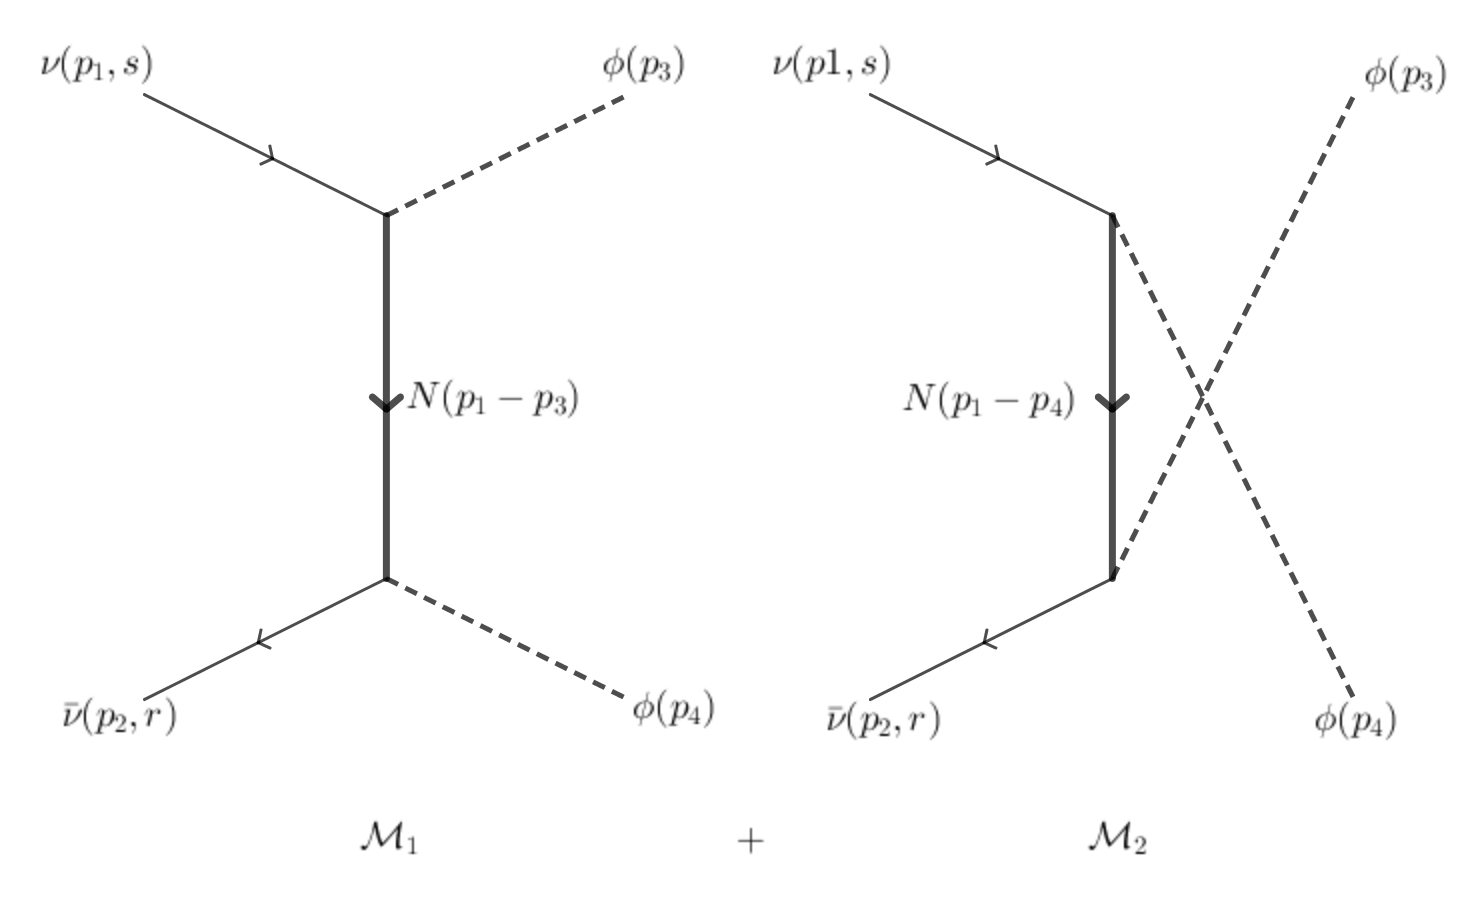
\includegraphics[width=0.6\linewidth]{feyndiag}
\caption{The two diagrams contributing to $\nu \bar{\nu} \rightarrow \phi \phi$ scattering amplitude in the case that $\phi$ is a real scalar and $\nu$, $N$ are Dirac fermions.}
\label{fig:feyn}
\end{framed}
\end{figure}
\subsection{Amplitudes}
\noindent Using the Feynman rules from the Lagrangian, we can write down the two amplitudes;
\begin{align}
-i\mM_1 &= \frac{g^2}{4}\bar{v}^r(\vec{p}_2)(1 - \gamma_5)\frac{\slashed{p}_1 - \slashed{p}_3 + m_N}{(p_1 - p_3)^2 - m_N^2}(1 - \gamma_5)u^s(\vec{p}_1) \\
-i\mM_2 &= \frac{g^2}{4}\bar{v}^r(\vec{p}_2)(1 - \gamma_5)\frac{\slashed{p}_1 - \slashed{p}_4 + m_N}{(p_1 - p_4)^2 - m_N^2}(1 - \gamma_5)u^s(\vec{p}_1)
\end{align}
We will need to compute the complex conjugate of this amplitude. If we consider;
\begin{equation*}
\mM \propto \bar{v}(1 - \gamma_5)(\slashed{k} + m_N)(1 - \gamma_5)u
\end{equation*}
along with the relations;
\begin{equation}
\gamma_\mu^{\dagger} = \gamma_0 \gamma_\mu \gamma_0, \,\, \gamma_5^{\dagger} = \gamma_5, \,\, \set{\gamma_\mu, \gamma_5} = 0
\end{equation}
then we find;
\begin{align*}
\mM^{\star} &= \left(v^{\dagger}\gamma_0(1 - \gamma_5)(k^{\mu}\gamma_\mu + m_N)(1 - \gamma_5)u\right)^{\star} \\
&= u^{\dagger}(1 - \gamma_5^{\dagger})(k^{\mu}\gamma_\mu^{\dagger} + m_N)(1 - \gamma_5^{\dagger})\gamma_0^{\dagger}v \\
&= u^{\dagger}\gamma_0(1 + \gamma_5)(k^{\mu}\gamma_\mu + m_N)(1 + \gamma_5)v \\
&= \bar{u}(1 + \gamma_5)(\slashed{k} + m_N)(1 + \gamma_5)v
\end{align*}
So we find that;
\begin{align}
i\mM_1^{\star} &= \frac{g^2}{4}\bar{u}^{s}(\vec{p}_1)(1 + \gamma_5)\frac{\slashed{p}_1 - \slashed{p}_3 + m_N}{(p_1 - p_3)^2 - m_N^2}(1 + \gamma_5)v^{r}(\vec{p}_2) \\
i\mM_2^{\star} &= \frac{g^2}{4}\bar{u}^{s}(\vec{p}_1)(1 + \gamma_5)\frac{\slashed{p}_1 - \slashed{p}_4 + m_N}{(p_1 - p_4)^2 - m_N^2}(1 + \gamma_5)v^{r}(\vec{p}_2)
\end{align}
\subsection{Squared Matrix Elements}
We can now compute the squared matrix elements;
\begin{multline*}
\left|\mM_1\right|^2 = \frac{g^4}{16}\left(\bar{u}^{s}(\vec{p}_1)(1 + \gamma_5)\frac{\slashed{p}_1 - \slashed{p}_3 + m_N}{(p_1 - p_3)^2 - m_N^2}(1 + \gamma_5)v^{r}(\vec{p}_2)\right) \\ \times \left(\bar{v}^r(\vec{p}_2)(1 - \gamma_5)\frac{\slashed{p}_1 - \slashed{p}_3 + m_N}{(p_1 - p_3)^2 - m_N^2}(1 - \gamma_5)u^s(\vec{p}_1) \right)
\end{multline*}
\begin{multline*}
\left|\mM_2\right|^2 = \frac{g^4}{16}\left(\bar{u}^{s}(\vec{p}_1)(1 + \gamma_5)\frac{\slashed{p}_1 - \slashed{p}_4 + m_N}{(p_1 - p_4)^2 - m_N^2}(1 + \gamma_5)v^{r}(\vec{p}_2)\right) \\ \times\left(\bar{v}^r(\vec{p}_2)(1 - \gamma_5)\frac{\slashed{p}_1 - \slashed{p}_4 + m_N}{(p_1 - p_4)^2 - m_N^2}(1 - \gamma_5)u^s(\vec{p}_1) \right)
\end{multline*}
\begin{multline*}
\mM_1^\star \mM_2 = \frac{g^4}{16}\left(\bar{u}^{s}(\vec{p}_1)(1 + \gamma_5)\frac{\slashed{p}_1 - \slashed{p}_3 + m_N}{(p_1 - p_3)^2 - m_N^2}(1 + \gamma_5)v^{r}(\vec{p}_2)\right) \\ \times\left(\bar{v}^r(\vec{p}_2)(1 - \gamma_5)\frac{\slashed{p}_1 - \slashed{p}_4 + m_N}{(p_1 - p_4)^2 - m_N^2}(1 - \gamma_5)u^s(\vec{p}_1) \right)
\end{multline*}
\begin{multline*}
\mM_2^\star \mM_1 = \frac{g^4}{16}\left(\bar{u}^{s}(\vec{p}_1)(1 + \gamma_5)\frac{\slashed{p}_1 - \slashed{p}_4 + m_N}{(p_1 - p_4)^2 - m_N^2}(1 + \gamma_5)v^{r}(\vec{p}_2)\right) \\ \times\left(\bar{v}^r(\vec{p}_2)(1 - \gamma_5)\frac{\slashed{p}_1 - \slashed{p}_3 + m_N}{(p_1 - p_3)^2 - m_N^2}(1 - \gamma_5)u^s(\vec{p}_1) \right)
\end{multline*}
The helicity averaged squared matrix element is then obtained via;
\begin{equation*}
\langle \Abs{\mM}^2 \rangle = \frac{1}{4}\sum_{r, s}{\left(\Abs{\mM_1}^2 + \mM_1^\star \mM_2 + \mM_2^\star \mM_1 + \Abs{\mM_2}^2\right)}
\end{equation*}
To do this sum we make use of the identities:
\begin{equation}
\sum_{r}{u_\alpha^r(\vec{p})\bar{u}_\beta^r(\vec{p})} = (\slashed{p} + m)_{\alpha \beta}, \,\, \sum_{r}{v_\alpha^r(\vec{p})\bar{v}_\beta^r(\vec{p})} = (\slashed{p} - m)_{\alpha \beta}
\end{equation}
We are working at energies much greater than the mass of the neutrino, so here $m_\nu = 0$. Hence;
\begin{align*}
\frac{1}{4}\sum_{r, s}{\left|\mM_1\right|^2 }&= \frac{g^4}{16}\tr\left[\slashed{p}_1(1 + \gamma_5)\frac{\slashed{p}_1 - \slashed{p}_3 + m_N}{(p_1 - p_3)^2 - m_N^2}(1 + \gamma_5)\slashed{p}_2(1 - \gamma_5)\frac{\slashed{p}_1 - \slashed{p}_3 + m_N}{(p_1 - p_3)^2 - m_N^2}(1 - \gamma_5) \right] \\
\frac{1}{4}\sum_{r, s}{\left|\mM_2\right|^2 }&= \frac{g^4}{16}\tr\left[\slashed{p}_1(1 + \gamma_5)\frac{\slashed{p}_1 - \slashed{p}_4 + m_N}{(p_1 - p_4)^2 - m_N^2}(1 + \gamma_5)\slashed{p}_2(1 - \gamma_5)\frac{\slashed{p}_1 - \slashed{p}_4 + m_N}{(p_1 - p_4)^2 - m_N^2}(1 - \gamma_5) \right] \\
\frac{1}{4}\sum_{r, s}{\mM_1^\star \mM_2}&= \frac{g^4}{16}\tr\left[\slashed{p}_1(1 + \gamma_5)\frac{\slashed{p}_1 - \slashed{p}_3 + m_N}{(p_1 - p_3)^2 - m_N^2}(1 + \gamma_5)\slashed{p}_2(1 - \gamma_5)\frac{\slashed{p}_1 - \slashed{p}_4 + m_N}{(p_1 - p_4)^2 - m_N^2}(1 - \gamma_5) \right] \\
\frac{1}{4}\sum_{r, s}{\mM_2^\star \mM_1}&= \frac{g^4}{16}\tr\left[\slashed{p}_1(1 + \gamma_5)\frac{\slashed{p}_1 - \slashed{p}_4 + m_N}{(p_1 - p_4)^2 - m_N^2}(1 + \gamma_5)\slashed{p}_2(1 - \gamma_5)\frac{\slashed{p}_1 - \slashed{p}_3 + m_N}{(p_1 - p_3)^2 - m_N^2}(1 - \gamma_5) \right] \\
\end{align*}
\subsection{Computing the Traces}
At this point we turn to the Dirac trace identities so as to do this analytically (in order to check the result obtained using \cite{Patel:2015tea}). We will make use of;
\begin{itemize}
\item $\tr(\gamma_{\mu}\gamma_{\nu}) = 4\eta_{\mu\nu}$
\item $\tr(\gamma_\mu \gamma_\nu \gamma_5) = 0$
\end{itemize}
as well as the fact that $\gamma_5^2 = \mathbb{I}_4$. Then we consider the general expression, which covers all the cases above;
\begin{align*}
&\tr\left[\slashed{p}_1(1 + \gamma_5)(\slashed{k}_1 + m_N)(1 + \gamma_5)\slashed{p}_2(1 - \gamma_5)(\slashed{k}_2 + m_N)(1 - \gamma_5)\right] \\
&\quad= p_1^{\mu}k_1^{\nu}p_2^{\rho}k_2^{\sigma}\tr\left[\gamma_\mu(1 + \gamma_5)\gamma_\nu(1 + \gamma_5)\gamma^{\rho}(1 - \gamma_5)\gamma^{\sigma}(1 - \gamma_5)\right] \\
&\qquad+ p_1^{\mu}k_1^{\nu}p_2^{\rho}m_N \tr\left[\gamma_\mu(1 + \gamma_5)\gamma_\nu(1 + \gamma_5)\gamma^{\rho}(1 - \gamma_5)(1 - \gamma_5)\right] \\
&\qquad \quad + p_1^{\mu}m_Np_2^{\rho}k_2^{\sigma} \tr\left[\gamma_\mu(1 + \gamma_5)(1 + \gamma_5)\gamma^{\rho}(1 - \gamma_5)\gamma_\sigma(1 - \gamma_5)\right] \\
&\qquad \qquad+ p_1^{\mu}p_2^{\rho}m_N^2 \tr\left[\gamma_\mu(1 + \gamma_5)(1 + \gamma_5)\gamma_\rho(1 - \gamma_5)(1 - \gamma_5)\right]
\end{align*}
Now, we first note the following;
\begin{align*}
\gamma_\mu (1 \pm \gamma_5)\gamma_\nu(1 \pm \gamma_5) &= \gamma_\mu(1 \pm \gamma_5)(1 \mp \gamma_5)\gamma_\nu \\
&= \gamma_\mu (\mathbb{I}_4 - \gamma_5^2)\gamma_\nu \\
&= 0
\end{align*}
So the first three terms vanish, we then just need to compute;
\begin{align*}
\tr\left[\gamma_\mu(1 + \gamma_5)(1 + \gamma_5)\gamma_\rho(1 - \gamma_5)(1 - \gamma_5)\right] &= 4\tr\left[\gamma_\mu(1 + \gamma_5)\gamma_\rho(1 - \gamma_5)\right] \\
&= 4\tr\left[\gamma_\mu \gamma_\rho (1 - \gamma_5)(1 - \gamma_5)\right] \\
&= 8\tr\left[\gamma_\mu \gamma_\rho (1 - \gamma_5)\right] \\
&= 32\eta_{\mu\rho}
\end{align*}
So we find that;
\begin{equation}
\tr\left[\slashed{p}_1(1 + \gamma_5)(\slashed{k}_1 + m_N)(1 + \gamma_5)\slashed{p}_2(1 - \gamma_5)(\slashed{k}_2 + m_N)(1 - \gamma_5)\right] = 32 m_N^2 (p_1 \cdot p_2)
\end{equation}
Therefore we find that;
\begin{align*}
\frac{1}{4}\sum_{r, s}{\left|\mM_1\right|^2 }&=  \frac{g^4}{64}32(p_1 \cdot p_2)m_N^2 \left(\frac{1}{(p_1 - p_3)^2 - m_N^2}\right)^2 \\
\frac{1}{4}\sum_{r, s}{\left|\mM_2\right|^2 }&=  \frac{g^4}{64}32(p_1 \cdot p_2)m_N^2 \left(\frac{1}{(p_1 - p_4)^2 - m_N^2}\right)^2 \\
\frac{1}{4}\sum_{r, s}{\mM_1^\star \mM_2}&=  \frac{g^4}{64}32(p_1 \cdot p_2)m_N^2 \left(\frac{1}{(p_1 - p_3)^2 - m_N^2}\right)\left(\frac{1}{(p_1 - p_4)^2 - m_N^2}\right) \\
\frac{1}{4}\sum_{r, s}{\mM_2^\star \mM_1}&=  \frac{g^4}{64}32(p_1 \cdot p_2)m_N^2 \left(\frac{1}{(p_1 - p_4)^2 - m_N^2}\right)\left(\frac{1}{(p_1 - p_3)^2 - m_N^2}\right) \\
\end{align*}
Summing these and using the definitions of the Mandelstam variables;
\begin{equation}
s = (p_1 + p_2)^2, \quad t = (p_1 - p_3)^2, \quad u = (p_1 - p_4)^2
\end{equation}
At this point, note that the expression for $s$ along with the fact that $p_1^2 = p_2^2 = m_\nu^2 \equiv 0$ gives;
\begin{equation*}
s = (p_1 + p_2)^2 = p_1^2 + p_2^2 + 2(p_1 \cdot p_2) = 2(p_1 \cdot p_2)
\end{equation*}
Then we can write down the helicity averaged squared matrix element;
\begin{examplebox1}
\begin{equation}
\label{eq:msquared}
\langle \Abs{\mM}^2 \rangle = \frac{1}{4} \sum_{r, s}{\Abs{\mM}^2} = \frac{1}{4}g^4 m_N^2 s \left(\left(\frac{1}{t - m_N^2}\right)^2 + \left(\frac{1}{u - m_N^2}\right)^2 + \frac{2}{(t - m_N^2)(u - m_N^2)}\right)
\end{equation}
\end{examplebox1}
\subsection{Kinematics}
To compute the integrated cross section, we need to consider the kinematics in the centre of mass frame. The general set up is shown in Figure \ref{fig:kinematics}. The following results and definitions hold in the centre of mass frame;
\begin{itemize}
\item $\vec{p}_1 + \vec{p}_2 = \vec{0}$ which implies $\vec{p}_3 + \vec{p}_4 = \vec{0}$ by conservation of $3$-momentum
\item Thus, $\Abs{\vec{p}_1} = \Abs{\vec{p}_2}$ and $\Abs{\vec{p}_3} = \Abs{\vec{p}_4}$
\item We define the scattering angle $\theta$ by $\vec{p}_1 \cdot \vec{p}_3 = \Abs{\vec{p}_1}\Abs{\vec{p}_3}\cos \theta$
\item Therefore, $\vec{p}_1 \cdot \vec{p}_4 = -\vec{p}_1 \cdot \vec{p}_3 =  -\Abs{\vec{p}_1}\Abs{\vec{p}_3}\cos \theta$
\end{itemize}
Conservation of energy with $m_\nu = 0$, along with $\Abs{\vec{p}_1} = \Abs{\vec{p}_2}$ and $\Abs{\vec{p}_3} = \Abs{\vec{p}_4}$ gives;
\begin{align*}
\Abs{\vec{p}_1} + \Abs{\vec{p}_2} &= \sqrt{\Abs{\vec{p}_3}^2 + m_\phi^2} + \sqrt{\Abs{\vec{p}_4}^2 + m_\phi^2} \\
\Rightarrow  \Abs{\vec{p}_1} &= \sqrt{\Abs{\vec{p}_3}^2 + m_\phi^2} \\
\Rightarrow  \Abs{\vec{p}_3} &= \sqrt{\Abs{\vec{p}_1}^2 - m_\phi^2}
\end{align*}
Furthermore, we have the $4$-momenta $p_1 = (\Abs{\vec{p}_1}, \vec{p}_1)$, $p_2 =  (\Abs{\vec{p}_1}, -\vec{p}_1)$, so $p_1 + p_2 = (2\Abs{\vec{p}_1}, \vec{0})$ which implies $s = (p_1 + p_2)^2 = 4\Abs{\vec{p}_1}^2$. Therefore we can read off;
\begin{equation}
\Abs{\vec{p}_1} = \frac{1}{2}\sqrt{s}, \quad \Abs{\vec{p}_3} = \sqrt{\frac{1}{4}s - m_\phi^2}
\end{equation}
\begin{figure}
\begin{framed}
 \centering
 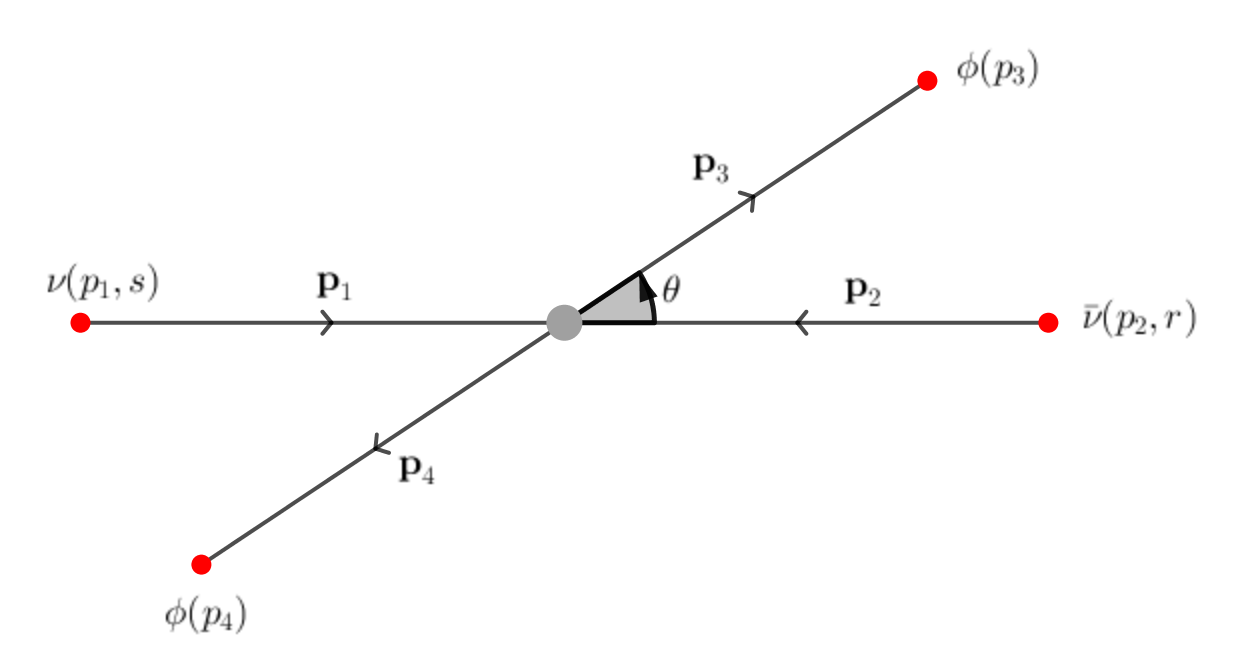
\includegraphics[width=0.6\linewidth]{comdiag}
 \caption{The kinematics in the centre of mass frame, acting as a definition of the scattering angle, $\theta$.}
 \label{fig:kinematics}
 \end{framed}
\end{figure}
We can then write the other Mandelstam variables in terms of only $s$ and $\theta$ as follows;
\begin{align*}
t &= (p_1 - p_3)^2 \\
&= p_1^2 + p_3^2 - 2 (p_1 \cdot p_3) \\
&= \underset{=0}{\underbrace{m_\nu^2}} + m_\phi^2 - 2(E_1 E_3 - \vec{p}_1 \cdot \vec{p}_3) \\
&= m_\phi^2 - 2\left(\Abs{\vec{p}_1}\sqrt{\Abs{\vec{p}_3}^2 + m_\phi^2} - \Abs{\vec{p}_1} \Abs{\vec{p}_3}\cos \theta\right) \\
&= m_\phi^2 - 2\left(\Abs{\vec{p}_1} \sqrt{\frac{1}{4}s - m_\phi^2 + m_\phi^2} - \Abs{\vec{p}_1}\sqrt{\frac{1}{4}s - m_\phi^2}\cos\theta\right) \\
&= m_\phi^2 - 2\left(\frac{1}{2}\sqrt{s}\cdot\frac{1}{2}\sqrt{s} - \frac{1}{2}\sqrt{s}\sqrt{\frac{1}{4}s - m_\phi^2}\cos\theta\right) \\
&= m_\phi^2 - \frac{1}{2}s + \sqrt{s\left(\frac{1}{4}s - m_\phi^2\right)}\cos\theta
\end{align*}
Finally we can use the relationship between the Mandelstam variables;
\begin{equation}
s + t + u = \sum_{i}{m_i^2} = 2m_\phi^2
\end{equation}
to write $u$ in terms of $s$ and $\theta$;
\begin{align*}
u &= 2 m_\phi^2 - s - t \\
&= 2 m_\phi^2 - s - m_\phi^2 + \frac{1}{2}s - \sqrt{s\left(\frac{1}{4}s- m_\phi^2 \right)}\cos\theta \\
&= m_\phi^2 - \frac{1}{2}s - \sqrt{s\left(\frac{1}{4}s - m_\phi^2\right)}\cos\theta
\end{align*}
Thus we can write the squared matrix element in terms of only $(s, \theta)$ as follows;
\begin{multline}
\langle \Abs{\mM}^2 \rangle = \frac{1}{4}g^4 m_N^2 s \left[ \frac{1}{\left(m_\phi^2 - m_N^2 - \frac{1}{2}s + \sqrt{s\left(\frac{1}{4}s - m_\phi^2\right)}\cos\theta\right)^2} \right. \\ \left. +  \frac{1}{\left(m_\phi^2 - m_N^2 - \frac{1}{2}s - \sqrt{s\left(\frac{1}{4}s - m_\phi^2\right)}\cos\theta\right)^2} \right. \\ \left. + \frac{2}{\left(m_\phi^2 - m_N^2 - \frac{1}{2}s + \sqrt{s\left(\frac{1}{4}s - m_\phi^2\right)}\cos\theta\right)\left(m_\phi^2 - m_N^2 - \frac{1}{2}s - \sqrt{s\left(\frac{1}{4}s - m_\phi^2\right)}\cos\theta\right)}  \right]
\end{multline}
\subsection{Method 1: The Differential Cross Section}
Our first method for computing the integrated cross section is via the differential cross section, which is given by the following standard result in the centre of mass frame, from \cite{Thomson:2013zua};
\begin{equation}
\frac{\ud \sigma}{\ud \Omega} = \frac{1}{64 \pi^2 s}\frac{\Abs{\vec{p}_3}}{\Abs{\vec{p}_1}} \langle \Abs{\mM}^2 \rangle
\end{equation}
Plugging in the expressions for $\Abs{\vec{p}_1}$ and $\Abs{\vec{p}_3}$ we therefore find;
\begin{multline*}
\frac{\ud \sigma}{\ud \Omega} = \frac{g^4 m_N^2}{256 \pi^2}\sqrt{\frac{s - 4m_\phi^2}{s}}\left[ \frac{1}{\left(m_\phi^2 - m_N^2 - \frac{1}{2}s + \sqrt{s\left(\frac{1}{4}s - m_\phi^2\right)}\cos\theta\right)^2} \right. \\ \left. +  \frac{1}{\left(m_\phi^2 - m_N^2 - \frac{1}{2}s - \sqrt{s\left(\frac{1}{4}s - m_\phi^2\right)}\cos\theta\right)^2} \right. \\ \left. + \frac{2}{\left(m_\phi^2 - m_N^2 - \frac{1}{2}s + \sqrt{s\left(\frac{1}{4}s - m_\phi^2\right)}\cos\theta\right)\left(m_\phi^2 - m_N^2 - \frac{1}{2}s - \sqrt{s\left(\frac{1}{4}s - m_\phi^2\right)}\cos\theta\right)}  \right]
\end{multline*}
To find the cross section we need to integrate over the solid angle;
\begin{equation}
\sigma = \int{\upd{\Omega}\frac{\ud \sigma}{\ud \Omega}} = \int_{0}^{2\pi}{\upd{\phi}\int_{-1}^{+1}{\upd{(\cos\theta)}\frac{\ud\sigma}{\ud \Omega}}} = 2\pi \int_{-1}^{+1}{\upd{(\cos\theta)}\frac{\ud\sigma}{\ud\Omega}}
\end{equation}
We make the following definitions to simplify the algebra;
\begin{itemize}
\item $\alpha = m_\phi^2 - m_N^2 - \frac{1}{2}s$
\item $\beta = \sqrt{s\left(\frac{1}{4}s - m_\phi^2\right)}$
\item $u = \cos\theta$
\end{itemize}
Then the cross section can be written as;
\begin{equation*}
\sigma = \frac{g^4 m_N^2}{128 \pi}\sqrt{\frac{s - 4m_\phi^2}{s}}\int_{-1}^{+1}{\upd{u}\left[\frac{1}{(\alpha + \beta u)^2} + \frac{1}{(\alpha - \beta u)^2} + \frac{2}{(\alpha - \beta u)(\alpha + \beta u)}\right]}
\end{equation*}
It remains to compute the integrals;
\begin{align*}
\int_{-1}^{+1}{\upd{u}\frac{1}{(\alpha + \beta u)^2}} &= \frac{1}{\beta}\left[-\frac{1}{\alpha + \beta u}\right]_{-1}^{+1} \\
&= \frac{2}{\alpha^2 - \beta^2} \\
\int_{-1}^{+1}{\upd{u}\frac{1}{(\alpha - \beta u)^2}} &=  \frac{2}{\alpha^2 - \beta^2} \\
\int_{-1}^{+1}{\upd{u}\frac{2}{(\alpha - \beta u)(\alpha + \beta u)}} &= \frac{2}{\alpha \beta}\log\left(\frac{\alpha + \beta}{\alpha - \beta}\right)
\end{align*}
So we find that;
\begin{equation*}
\sigma = \frac{g^4 m_N^2}{128 \pi}\sqrt{\frac{s - 4m_\phi^2}{s}}\left(\frac{4}{\alpha^2 - \beta^2} + \frac{2}{\alpha \beta}\log\left(\frac{\alpha + \beta}{\alpha - \beta}\right)\right)
\end{equation*}
Substituting our expressions for $\alpha$ and $\beta$ from above we find;
\begin{multline*}
\sigma = \frac{g^4 m_N^2}{64\pi}\sqrt{\frac{s - 4m_\phi^2}{s}}\left( \frac{2}{\left(m_\phi^2 - m_N^2 - \frac{1}{2}s\right)^2 - s\left(\frac{1}{4}s - m_\phi^2\right)} \right. \\ \left. + \frac{1}{\left(m_\phi^2 - m_N^2 - \frac{1}{2}s\right)\sqrt{s\left(\frac{1}{4}s - m_\phi^2\right)}} \log\left(\frac{m_\phi^2 - m_N^2 - \frac{1}{2}s + \sqrt{s\left(\frac{1}{4}s - m_\phi^2\right)}}{m_\phi^2 - m_N^2 - \frac{1}{2}s - \sqrt{s\left(\frac{1}{4}s - m_\phi^2\right)}}\right)\right)
\end{multline*}
which reduces to;
\begin{examplebox1}
\begin{multline}
\label{eq:sigma}
\sigma(s) = \frac{g^4 m_N^2}{32 \pi}\left[\sqrt{\frac{\frac{1}{4}s - m_\phi^2}{s}}\frac{2}{\left(m_\phi^2 - m_N^2 - \frac{1}{2}s\right)^2 - s\left(\frac{1}{4}s - m_\phi^2\right)} \right. \\ \left. + \frac{1}{s\left(m_\phi^2 - m_N^2 - \frac{1}{2}s\right)}\log\left(\frac{m_\phi^2 - m_N^2 - \frac{1}{2}s + \sqrt{s\left(\frac{1}{4}s - m_\phi^2\right)}}{m_\phi^2 - m_N^2 - \frac{1}{2}s - \sqrt{s\left(\frac{1}{4}s - m_\phi^2\right)}}\right)\right]
\end{multline}
\end{examplebox1}
\subsection{Method 2: Integrating over $t$}
As a check of the integration, we want to see that we obtain the same result by instead integrating over the Mandelstam variable $t$. Again, we use a standard result from \cite{Thomson:2013zua};
\begin{equation}
\frac{\ud \sigma}{\ud t} = \frac{1}{64 \pi s \Abs{\vec{p}_1}^2}\langle \Abs{\mM}^2 \rangle
\end{equation}
Using again the fact that $\Abs{\vec{p}_1} = \frac{1}{2}\sqrt{s}$ we see that;
\begin{equation*}
\sigma = \int_{t_0}^{t_1}{\upd{t}\frac{\langle \Abs{\mM}^2 \rangle}{16 \pi s^2}}
\end{equation*}
To determine the limits on the integration we consider the expression from the Kinematics section;
\begin{equation*}
t = m_\phi^2 - \frac{1}{2}s + \sqrt{s\left(\frac{1}{4}s - m_\phi^2\right)}\cos\theta
\end{equation*}
The extremal values occur when $\cos\theta = \pm 1$, so we find;
\begin{equation}
t_0 = m_\phi^2 - \frac{1}{2}s - \sqrt{s\left(\frac{1}{4}s - m_\phi^2\right)}, \,\, t_1 = m_\phi^2 - \frac{1}{2}s + \sqrt{s\left(\frac{1}{4}s - m_\phi^2\right)}
\end{equation}
We can write the matrix element in terms of only $s$ and $t$ using $s + t + u = 2m_\phi^2$, then substituting this into \eqref{eq:msquared} we find;
\begin{equation*}
\frac{\langle \Abs{\mM}^2 \rangle}{16\pi s^2} = \frac{g^4 m_N^2}{64\pi s}\left(\left(\frac{1}{t - m_N^2}\right)^2 + \left(\frac{1}{2m_\phi^2 - m_N^2 - s - t}\right)^2 + \frac{2}{(t - m_N^2)(2m_\phi^2 - m_N^2 - s - t)}\right)
\end{equation*}
We can then gather together some integrals, firstly;
\begin{equation*}
\int_{t_0}^{t_1}{\upd{t}\frac{1}{(t - a)^2}} = \frac{1}{t_0 - a} - \frac{1}{t_1 - a}
\end{equation*}
which we apply with $a = m_N^2$ and $a = 2m_\phi^2 - m_N^2 - s$ to find;
\begin{multline*}
\int_{t_0}^{t_1}{\upd{t}\left(\frac{1}{(t - m_N^2)^2} + \frac{1}{(2m_\phi^2 - m_N^2 - s - t)^2}\right)} \\ = \frac{1}{m_\phi^2 - m_N^2 - \frac{1}{2}s - \sqrt{s\left(\frac{1}{4}s - m_\phi^2\right)}} - \frac{1}{m_\phi^2 - m_N^2 - \frac{1}{2}s + \sqrt{s\left(\frac{1}{4}s - m_\phi^2\right)}} \\ + \frac{1}{m_\phi^2 - 2m_\phi^2 + m_N^2 + s - \frac{1}{2}s - \sqrt{s\left(\frac{1}{4}s - m_\phi^2\right)}} \\ - \frac{1}{m_\phi^2 - 2m_\phi^2 + m_N^2 + s - \frac{1}{2}s + \sqrt{s\left(\frac{1}{4}s - m_\phi^2\right)}}
\end{multline*}
Simplifying the last two terms we find;
\begin{align*}
&\int_{t_0}^{t_1}{\upd{t}\left(\frac{1}{(t - m_N^2)^2} + \frac{1}{(2m_\phi^2 - m_N^2 - s - t)^2}\right)} \\
&\qquad \qquad= \frac{2}{m_\phi^2 - m_N^2 - \frac{1}{2}s - \sqrt{s\left(\frac{1}{4}s - m_\phi^2\right)}} - \frac{2}{m_\phi^2 - m_N^2 - \frac{1}{2}s + \sqrt{s\left(\frac{1}{4}s - m_\phi^2\right)}} \\
&\qquad \qquad= \frac{4\sqrt{s\left(\frac{1}{4}s - m_\phi^2\right)}}{\left(m_\phi^2 - m_N^2 - \frac{1}{2}s\right)^2 - s\left(\frac{1}{4}s - m_\phi^2\right)}
\end{align*}
The last integral can be evaluated by considering;
\begin{align*}
\int_{t_0}^{t_1}{\upd{t}\frac{1}{(t - a)(b - t)}} &= \int_{t_0}^{t_1}{\upd{t}\frac{1}{b - a}\left(\frac{1}{t - a} + \frac{1}{b - t}\right)} \\
&= \frac{1}{b - a}\left[\log\left(\frac{t - a}{b - t}\right)\right]_{t_0}^{t_1} \\
&= \frac{1}{b - a}\log\left(\frac{(t_1 - a)(b - t_0)}{(b - t_1)(t_0 - a)}\right)
\end{align*}
We apply this with $a = m_N^2$, $b = 2m_\phi^2 - m_N^2 - s$ which gives;
\begin{align*}
&\frac{1}{2m_\phi^2 - 2m_N^2 - s}\log\left( \frac{\left(m_\phi^2 - m_N^2 -\frac{1}{2}s + \sqrt{s\left(\frac{1}{4}s - m_\phi^2\right)}\right)}{\left(2m_\phi^2 - m_N^2 - s - m_\phi^2 + \frac{1}{2}s - \sqrt{s\left(\frac{1}{4}s - m_\phi^2\right)}\right)} \right. \\
& \qquad \quad \cdot \left. \frac{\left(2m_\phi^2 - m_N^2 - s - m_\phi^2 + \frac{1}{2}s +  \sqrt{s\left(\frac{1}{4}s - m_\phi^2\right)}\right)}{\left(m_\phi^2 - m_N^2 -\frac{1}{2}s - \sqrt{s\left(\frac{1}{4}s - m_\phi^2\right)}\right)}\right) \\
&\quad=\frac{1}{2m_\phi^2 - 2m_N^2 - s} \log\left(\frac{\left(m_\phi^2 - m_N^2 -\frac{1}{2}s + \sqrt{s\left(\frac{1}{4}s - m_\phi^2\right)}\right)^2}{\left(m_\phi^2 - m_N^2 -\frac{1}{2}s - \sqrt{s\left(\frac{1}{4}s - m_\phi^2\right)}\right)^2}\right) \\
&\quad=\frac{1}{m_\phi^2 - m_n^2 - \frac{1}{2}s}\log\left(\frac{m_\phi^2 - m_N^2 - \frac{1}{2}s + \sqrt{s\left(\frac{1}{4}s - m_\phi^2\right)}}{m_\phi^2 - m_N^2 - \frac{1}{2}s - \sqrt{s\left(\frac{1}{4}s - m_\phi^2\right)}}\right)
\end{align*}
Adding the two integrals together and collecting the terms, we do indeed recover the expression in \eqref{eq:sigma}.

\section{Results}
\begin{figure}
\begin{framed}
 \centering
 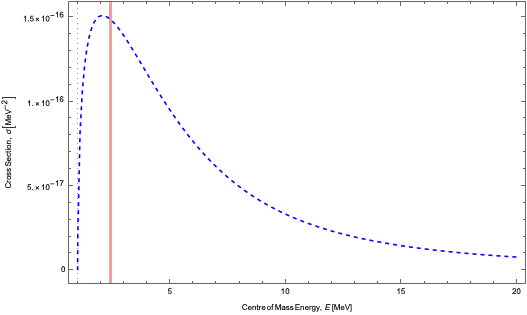
\includegraphics[width=0.7\linewidth]{sigma}
 \caption{The interaction cross section $\sigma(s)$ plotted with the values of the parameters given by $m_\nu = 0.01 \, \text{eV}, g = 10^{-3}$, $m_\phi = 1 \, \text{MeV}$, $m_N = 10 \, \text{MeV}$. The black dotted line indicates the threshold energy at $m_\phi$, whilst the thick red line indicates the centre of mass energy of the PeV neutrino.}
 \label{fig:sigmaplot}
\end{framed}
\end{figure}
\subsection{Plotting the Cross Section}
We now look to check our result by making some initial plots and comparing the centre of mass energy for the original PeV neutrino. We assume that the neutrino from the blazar has an energy $E_\nu = 1 \, \text{PeV}$ and that the cosmic neutrino background is approximately at rest. Then, the energy of the blazar neutrino in the centre of mass frame is given by $E^\star_\nu = \sqrt{2m_\nu E_\nu}$ which is $\mO(\text{MeV})$. We note that this depends on the neutrino mass, but more importantly is $\mO(m_\phi, m_N)$. There are a number of things to note from Figure \ref{fig:sigmaplot};
\begin{itemize}
\item The threshold centre of mass energy, at the mass of the scalar, for the creation of the two $\phi$ particles is indeed realised in our analytic expression
\item Whilst the neutrinos from the blazar are very high energy, the small value of the neutrino mass (taken here to be $0.01 \, \text{eV}$) actually ensures that the centre of mass energy of the collision is precisely around the resonance peak. It could therefore be argued perhaps that the process is interesting precisely because the neutrinos have such a high energy. If they had a smaller energy, the centre of mass energy would be below the threshold and the process could not occur.
\end{itemize}
\subsection{What next?}
Now we have the cross section, we need to try and put some constraints on the model via some astrophysical considerations. These might include;
\begin{itemize}
\item Using the cross section to calculate the mean free path for the neutrino from the blazar, this might involve integrating over the dark matter density, $n_\chi(z)$.
\item The blazar is $\sim 5.6$ billion light years away, so a red shift in the neutrino energy may be important, indeed the red shift might cause the effective energy at some red shift, $z$, to fall below the threshold energy discussed above. If this is the case, then there will be a cutoff $z^\star$, after which the process will not happen.
\item Whether we need to consider other scattering channels, off e.g. dark matter to calculate the mean free path.
\item How to combine the above to put constraints on the model, including which variables to constrain ($m_\phi, m_N$ etc.).
\end{itemize}









\hrule
\vspace{1pt}
\hrule
\nocite{*}
\bibliography{update7Nov}
\vspace{15pt}
\hrule
\vspace{1pt}
\hrule
\end{document}
